\documentclass[11pt, oneside,titlepage]{article}   	% use "amsart" instead of "article" for AMSLaTeX format
\usepackage{geometry}                		% See geometry.pdf to learn the layout options. There are lots.
\geometry{letterpaper}                   		% ... or a4paper or a5paper or ... 
%\geometry{landscape}                		% Activate for rotated page geometry
\usepackage[parfill]{parskip}    		% Activate to begin paragraphs with an empty line rather than an indent
\usepackage{graphicx}				% Use pdf, png, jpg, or eps§ with pdflatex; use eps in DVI mode
								% TeX will automatically convert eps --> pdf in pdflatex		
								
\usepackage{amsmath}
\usepackage{amssymb}
\usepackage{amsmath}
\usepackage{mathabx}
\usepackage[ruled]{algorithm2e}
\usepackage{hyperref}
\usepackage{placeins}

\title{CS267 Final Project Report\\
  \large Parallelizing Empirical Variograms for Large Data Sets\\
  \url{https://github.com/hsavoy/cs267FinalProject}}
\author{Andreas Borgen Longva\\
  \texttt{longva@berkeley.edu}
  \and
  Heather Savoy\\
  \texttt{frystacka@berkeley.edu}}
\date{May 11, 2015}							% Activate to display a given date or no date

\begin{document}
\maketitle
\section{Project Description}
%What is a variogram, its application, why not yet parallel, comparison to particle simulation
%Note on how this will actually be used in research
%How we tested for correctness


The field of geostatistics strives to characterize the spatial heterogeneity found in the physical world in terms of probability and statistics. A common method to represent how values of a field are correlated over space is called a variogram. The variogram is a function of distance between points in space and describes the increase in variance between points as distance grows. The shape of a variogram is highly informative for gauging the heterogeneity of a spatial field. For example, the near-origin slope of the variogram indicates if values change smoothly or sharply across the field. 

One important application of variograms is in groundwater modeling. Measuring hydraulic properties of aquifers is difficult because most methods involve drilling into the subsurface, which is expensive and destructive. Measurements are often scarce and modelers have traditionally averaged their sparse data to assign constant values in their numerical models, however studies have shown that certain subsurface processes are highly dependent on aquifer heterogeneity. Variograms are used to construct covariance matrices of multi-normal distributions which are sampled to create realizations of random heterogeneous fields. An ensemble of these random fields can be used to study subsurface processes in a stochastic fashion.      

To estimate a field site's variogram, measurements are used to construct an empirical variogram: 
\begin{equation}
\hat{\gamma}(h)=\frac{1}{2|N(h)|}\sum_{(i,j)\in N(h)} |z_i-z_j|^2
\end{equation}
where $h$ is distance between two points in space ($i$ and $j$), the value of the field at point $i$ is $z_i$, $N(h)$ is the group of pairs of points separated by distance $h$, and $|N(h)|$ is the number of pairs in the group. Geostatistical software packages exist to convert spatial data measurements into empirical variograms already, but they are designed for small data sets. Since most field site's only have between $10^1 - 10^3$ data points, the straight-forward $O(n^2)$ algorithm for calculating the empirical variogram is computationally feasible. However, current research is being conducted with three-dimensional aquifer analogs to understand realistic heterogeneities given fully known domains. Figure~\ref{fig:herten} is a visualization of such a data set and it contains $8.96\times 10^6$ data points which creates $4\times 10^13$ pairs to consider in the empirical variogram calculation. Using the traditional geostatistical packages on a personal computer for this data set would require an unreasonable amount of time (on the order of weeks). Thus, we chose to pursue the empirical variogram calculation for large data sets as our project.   

\begin{figure}[!ht]
   \centering
   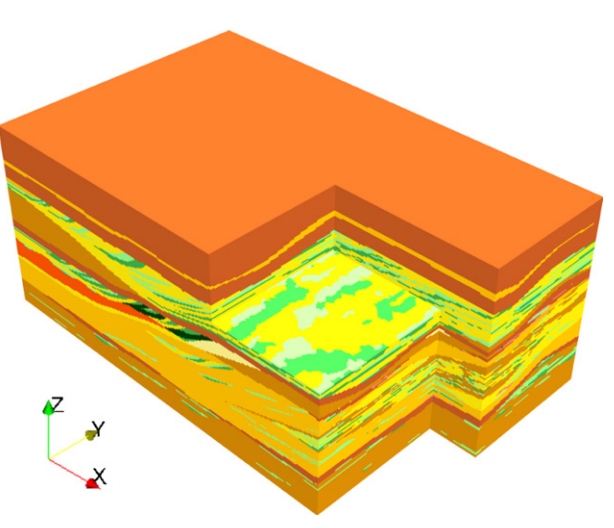
\includegraphics{./fig/herten.png} % requires the graphicx package
   \caption{A visualization of a three-dimensional aquifer analog. The domain covers 16x10x7m at 5cm resolution. The color indicates soil type, which influences groundwater flow and contaminant transport processes. (Copied from \cite{Comunian2011a})}
   \label{fig:herten}
\end{figure}




\section{Implementations}
%Overview of different implementations and their goals ?
%Any assumptions we made for all?
  \subsection{Serial}
    %Brief description
%pseudo-code
%Expected performance
 % \subsection{Naive MPI}
  %  %Brief description
%pseudo-code
%Expected performance
  \subsection{Communication Optimal Non-symmetric Algorithm}
    %Brief description
%pseudo-code
%Expected performance
Driscoll et al. \cite{Driscoll2013} presented a communicational-optimal algorithm for computing all-pairs N-body interactions. The algorithm is a variation of the more well-known cyclic shifting algorithm. Here they introduced the concept of a replication factor, $c$, which essentially has the effect of reducing the total communication required by trading parts of the point-to-point communication for broadcasts, which are asymptotically more efficient. This comes at the expense of a factor $c$ higher memory usage.

We implemented a variant of this algorithm, modified to fit the pattern of the empirical variogram computation. The resulting algorithm is presented is presented in \ref{alg:commopt}. Given $P$ processors, the processors are arranged in a $c \times \frac{P}{c}$ grid, where each column represents a \emph{team}. For each team, the processor in the given column at the top of the row is designated as a team leader. The set of all data points is evenly distributed among the team leaders. 

Next, each team leader determines the minimum bounding box (or rectangle, depending on dimensions) that covers all the data points associated with the team. A global minimum bounding box is obtained by min-max all-reduction across team leaders. The diagonal of this global bounding box is used as the maximum distance between any two data points. The data points associated with each team, as well as the maximum distance, is then broadcast from the team leader to the rest of the team. 

At this point, each processor copies his set of local points to an exchange buffer, and \emph{shifts} his exchange buffer by $i$, where $i$ is the processor's row in the grid. Consider a processor in row $i$ and column $j$, denoted $(i, j)$. The $\text{shift}(k)$ procedure sends the data in the exchange buffer of processor $(i, j)$ to the processor in the same row with column $(j + k \mod P / c)$, and receives data from column $(j - k \mod P / c)$ and stores it in the exchange buffer. In other words, it is a cyclic shift along row $i$. 

Each processor $(i, j)$ performs an \emph{initial shift} by calling $\text{shift}(i)$. This is followed by $P / c^2$ iterations, for which each processor calls $\text{shift}(c)$ and subsequently computes interactions between its local buffer and its exchange buffer, as in the serial case.

Finally, all processors participate in a sum-reduction of the binned semivariance data, and the root node completes the variogram by dividing each bin by $2 N_b$, where $N_b$ is the number of elements in the distance bin $b$.

\begin{algorithm}[H]
 \DontPrintSemicolon
 \KwIn{Replication factor $c$}
 \KwIn{P processors arranged in a $c \times \frac{P}{c}$ grid }
 \KwIn{A set S of data points distributed evenly among team leaders into subsets $S_t$}
 \KwIn{B, the number of distance bins to use in variogram computation}
 \KwOut{$\gamma(b)$ for $b = 1, ..., B$}

 \tcp{In parallel on all processors} 
 
 $\gamma \gets \text{zero-initialized array of size B}$ \;
 $N \gets \text{zero-initialized array of size B}$ \;
  
 \If{team leader}{
	$\text{bounds} \gets \operatorname{minimum-bounding-box}(S_t)$ \;
	all-reduce(bounds) among team leaders \;
	$d_{\max} \gets \text{diagonal}(\text{bounds})$
 }
 
 Broadcast $S_t$, $d_{\max}$ from team leaders to team \;
 $\text{local}$, $\text{buffer}$ $\gets S_t$
 
 \For{$p / c^2$ iterations} {
    shift(buffer, c) \;
	\ForEach{$(i, j) \in \text{local} \times \text{buffer}$}
	{
        $d \gets \operatorname{dist}(i, j)$ \;
        $b \gets \operatorname{bin}(d)$ \;
		$\gamma[b] \gets \gamma[b] + |z_i - z_j|^2$ \;
		$N[b] \gets N[b] + 1$ \;
	}
 }
 
 $\gamma, N \gets \text{sum-reduce across all processors to root node}$ \;
 $\gamma \gets \gamma[b] / (2 \cdot N[b]), \quad b = 1, ..., B$\;
 \caption{Communication-optimal Non-symmetric Algorithm}
 \label{alg:commopt}
\end{algorithm}
  \subsection{Computation Optimal Algorithm}
   %Brief description
%pseudo-code
%Expected performance

\cite{Koanantakool}
   
   \FloatBarrier
\section{Results}
  %Plot of n versus time for all implementations
%Effect of tuning parameters (how many copies?)
%Extrapolation of how long my data set would take with each?
%Actual result for my data set

We created a series of test cases of various sizes and ran our different implementations on Hopper. We checked the correctness of our implementations by comparing our results to results given by the R package \texttt{gstat} \cite{Pebesma} for the smaller test cases.

\begin{figure}[!h]
   \centering
   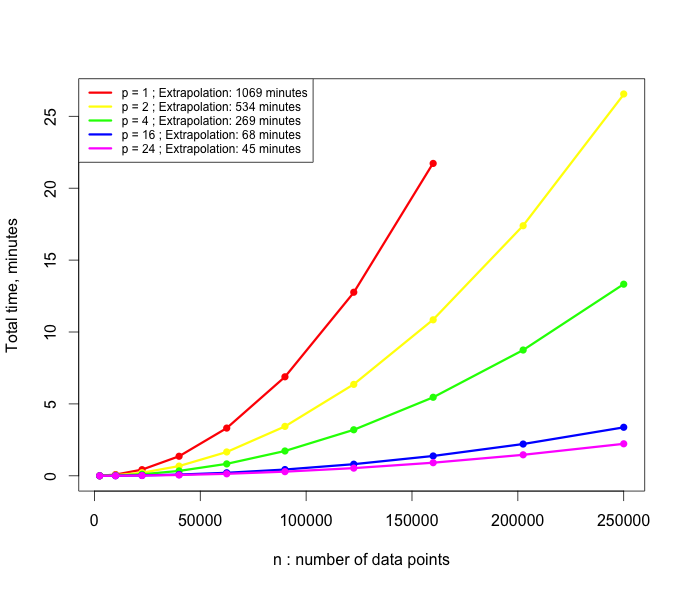
\includegraphics[width=0.75\textwidth]{./fig/comm_c1_timings.png} % requires the graphicx package
   \caption{For all 10 test cases, various numbers of processors in one node were timed and the curves represent the number of processors. A line was fit for the square root of time versus test case size and extrapolated to $n=8.69\times10^6$, the result listed in the legend). For this communication optimal implementation on one node, the large data set is still not reasonable.}
   \label{fig:comm_c1_timings}
\end{figure}

We executed 10 test cases for our communication-optimal and computational-optimal implementations for various numbers of processors. Figure~\ref{fig:comm_c1_timings} shows the timing results for our communication optimal implementation with the replication factor $c=1$. It depicts the distinctive $O(n^2)$ curve for the smaller number of processors $p$ (the horizontal axis is too small to show the shape of the curve for the larger $p$) and the expected reduction in time with increasing $p$. For each of these curves, we fit a line between total time and $n^2$ and then extrapolated the time required to run the large dataset of Figure~\ref{fig:herten} with $n=8.69\times10^6$. On the legend, the extrapolated time is written for each $p$ tested.  

Figure~\ref{fig:comm_allc_timings} compares $c=$ 1, 2, and 4. The effect of $c$ is not evident when looking at the total time. When breaking the total time down into time for reading the file, broadcasting the point data, shifting the point data, computing the squared differences, and reducing the bins (see Figure~\ref{fig:allc_breakdown}), it is evident that most of the total time is consumed by the computation stage. The effect of $c$ is more evident if only the shifting time is plotted (see Figure~\ref{fig:comm_allc_comm})

\begin{figure}[!h]
   \centering
   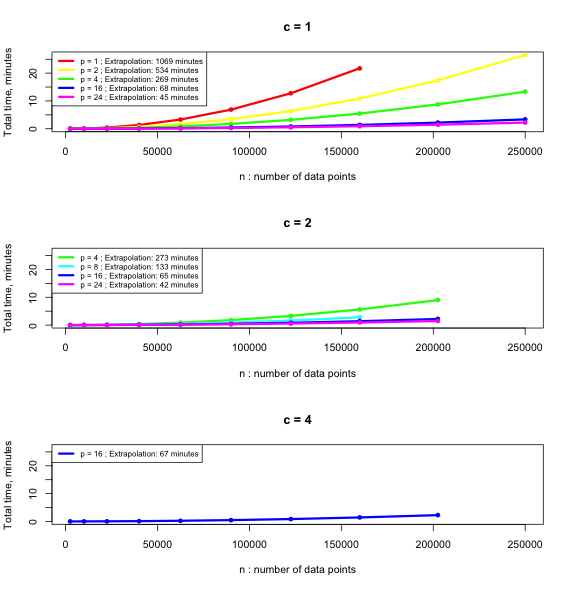
\includegraphics[width=\textwidth]{./fig/comm_allc_timings.png} % requires the graphicx package
   \caption{For all 10 test cases, various numbers of processors in one node were timed and the curves represent the number of processors. there is no detectable difference for the different values of $c$. }
   \label{fig:comm_allc_timings}
\end{figure}

\begin{figure}[!h]
   \centering
   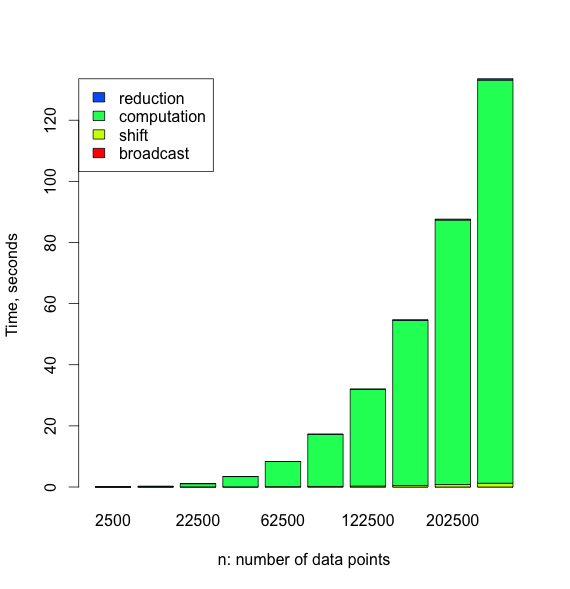
\includegraphics[width=0.75\textwidth]{./fig/comm_24_breakdown.png} % requires the graphicx package
   \caption{The breakdown of total time for executing our communication optimal code for 24 processors. The categories considered are shifting the data points, broadcasting the points, calculating the square differences, and reducing the bins. The collective communication calls of broadcast and reduce are effectively zero and computation dominates. }
   \label{fig:allc_breakdown}
\end{figure}

\begin{figure}[!h]
   \centering
   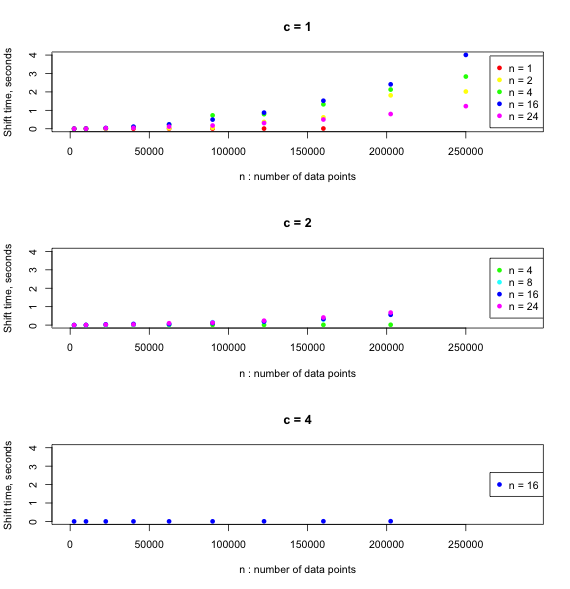
\includegraphics[width=\textwidth]{./fig/comm_allc_comm.png} % requires the graphicx package
   \caption{The time for shifting the data points around the processor teams in the communication optimal implementation is shown for different test case size and number of processors. With increasing $c$, the shifting time reduces, but there are less options for $p$ since $c^2$ needs to divide $p$ evenly. The effect of the replication factor $c$ is only seen for the shifting time and none of the other timing categories, however since computation out weighs communication the $c$ is not a tuning parameter we spent much time configuring.}
   \label{fig:comm_allc_comm}
\end{figure}

Due to computation consuming most of the total time, we next tried the computation optimal implementation. Figure~\ref{fig:comp_timings} shows the timing results for total time of our 10 test cases and for a range of processors. Again, the $O(n^2)$ curve is evident and we extrapolated the time required for our large data set. The total time for the computation optimal implementation is about half of that of the communication optimal implementation. Breaking down the total time for this computation optimal implementation (Figure~\ref{fig:comp_breakdown}), we can see that reading the input becomes the bottle neck  when increasing the number of processors. Note that the timing numbers for input reading includes an all-reduce to distribute the global minimum bounding box across all processors, which may be part of the reason the time for reading is noticably higher for $p = 240$ compared to $p = 2$.

\begin{figure}[!h]
   \centering
   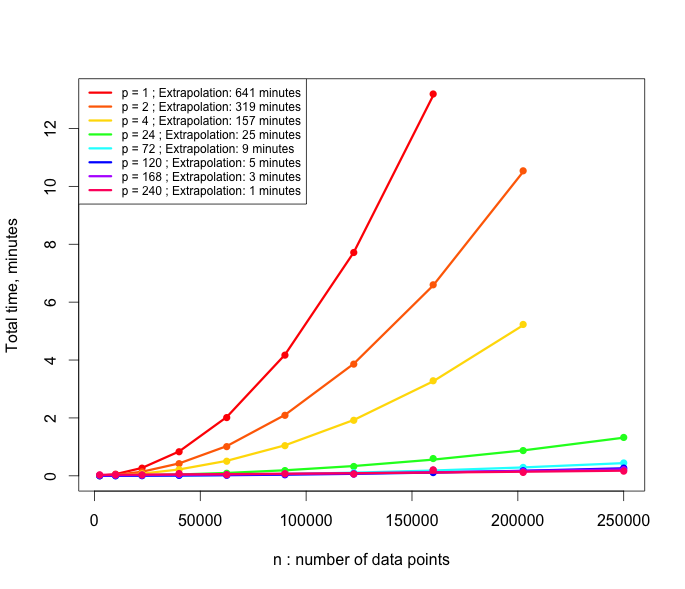
\includegraphics[width=0.75\textwidth]{./fig/timing.png} % requires the graphicx package
   \caption{For all 10 test cases, various numbers of processors in one node were timed and the curves represent the number of processors. A line was fit for the square root of time versus test case size and extrapolated to $n=8.69\times10^6$, the result listed in the legend). As to be expected, increasing the number of processors lowered the total time for each test case, and the effect is more pronounced with larger test cases. Although it doesn't appear that increasing the number of processors helps much after $p=72$, the effect would be more pronounced for cases larger than our test cases. }
   \label{fig:comp_timings}
\end{figure}

\begin{figure}[!h]
   \centering
   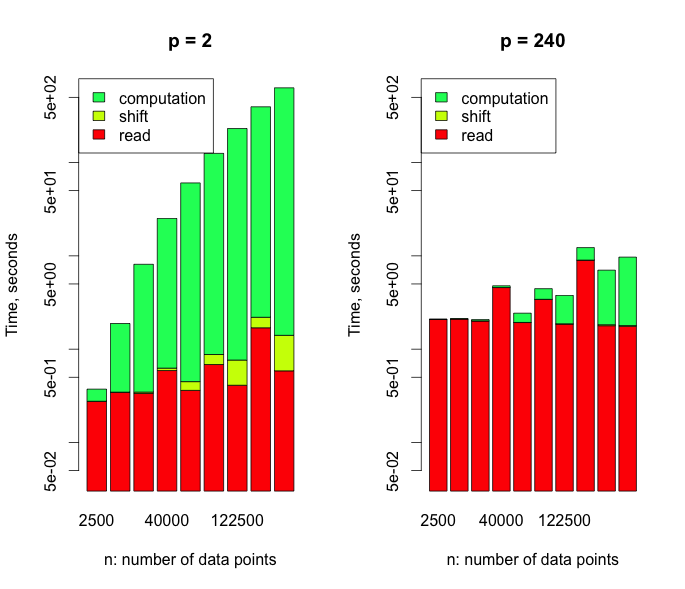
\includegraphics[width=0.75\textwidth]{./fig/comp_breakdown.png} % requires the graphicx package
   \caption{The log-scale breakdown of total time for executing our computation optimal code for 2 and 240 processors. The three categories considered are reading the file, shifting the data points, and calculating the square differences. The collective communication calls of broadcast and reduce are not included as they were effectively zero. For $p=2$ computation dominates, but for $p=240$, reading the file dominates.}
   \label{fig:comp_breakdown}
\end{figure}

Next, we looked at the scaling success (Figure~\ref{fig:scaling}). We divided the time $p=1$ by each larger $p$ and compared it to the $y=x$ line representing perfect scaling. It can be seen that for the larger test cases, there is near-perfect scaling for up to 144 processors. Although this is not the case for the smaller test cases, this is not really an issue because our program is designed for large data sets and small ones can be run in serial in reasonable time. 

\begin{figure}[!h]
   \centering
   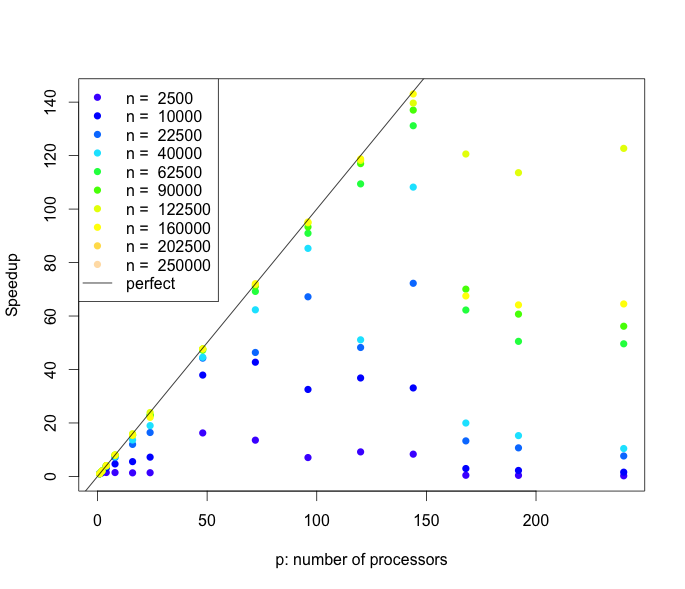
\includegraphics[width=0.75\textwidth]{./fig/speedup.png} % requires the graphicx package
   \caption{For all 10 test cases, various numbers of processors were timed and compared to the $p=1$ case for the respective test case size. larger test cases exhibit better scaling than smaller test cases, and using up to 144 processors showed near-perfect scaling.}
   \label{fig:scaling}
\end{figure}

Next, we increased $p$ and re-ran our test cases to determine the appropriate $p$ to run our large data set in around an hour (instead of a day which is the quickest we could get with one node in our preliminary tests). Figure~\ref{fig:extrapolate} shows the extrapolated time for the large data set for increasing number of nodes (each with 24 processors).

\begin{figure}[!h]
   \centering
   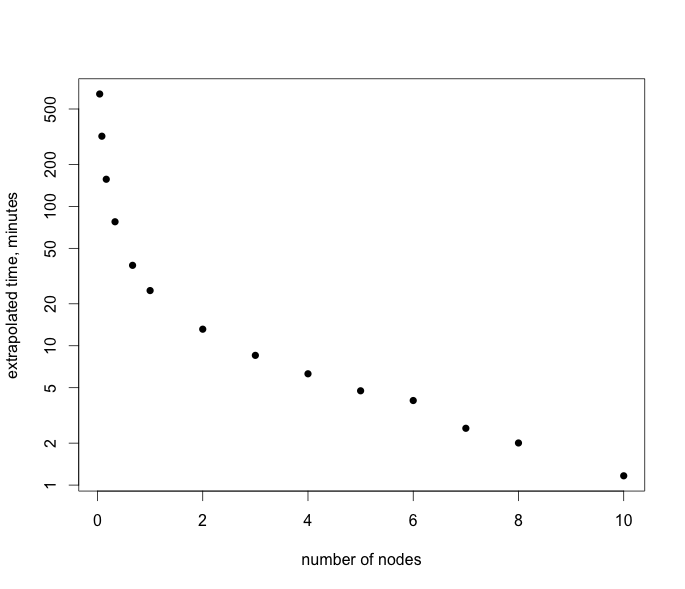
\includegraphics[width=0.75\textwidth]{./fig/extrapolate.png} % requires the graphicx package
   \caption{The log-scale extrapolated time to calculate the empirical variogram for $n=8.69\times10^6$ from a few processors in one node up to all 24 processors in 10 nodes. With the 10 nodes, it will only take one minute to calculate the variogram.}
   \label{fig:extrapolate}
\end{figure}


   \FloatBarrier
\section{Conclusion}
   %Which implementation(s) worked best? Always the case?
%What can be learned from the results to my dataset
%How this can be made more general (for future applications)
%Can now fit models and make simulations (for which algorithms already exist)
   
   \FloatBarrier

\bibliographystyle{plain}
\bibliography{ref}


\end{document}  
